\documentclass{article}

\usepackage{iclr2026/iclr2026_conference,times}
\input{iclr2026/math_commands.tex}

\usepackage{hyperref}
\usepackage{url}
\usepackage{booktabs}
\usepackage{amsfonts}
\usepackage{amsmath}
\usepackage{nicefrac}
\usepackage{microtype}
\usepackage{xcolor}
\usepackage{graphicx}
\usepackage{algorithm}
\usepackage{algorithmic}
\usepackage{multirow}

\title{Speculative Recommendation Serving:\\Accelerating Inference via Multi-Cluster Draft-and-Verify}

\author{Anonymous}

\iclrfinalcopy

\begin{document}

\maketitle

\begin{abstract}
We propose \textbf{speculative recommendation serving}, a framework that accelerates recommendation inference by borrowing the draft-and-verify paradigm from speculative decoding in large language models. Given a user request, our system \emph{drafts} candidate recommendations from the $K$ nearest user-cluster caches, \emph{verifies} each draft via a score-ratio acceptance criterion that mirrors the token-level acceptance probability in speculative decoding, and either \emph{accepts} the best-matching draft or falls back to fresh computation. On MovieLens-1M, multi-cluster speculation ($K$=3) achieves an 89\% acceptance rate with 8$\times$ estimated speedup while retaining 83\% of fresh-model NDCG@10. Critically, 55\% of accepted results are served by a \emph{non-nearest} cluster---a phenomenon we term \textbf{multi-cluster gain}---demonstrating that speculating across multiple clusters recovers users who would otherwise be rejected by their nearest cluster alone. We present the first formal connection between speculative decoding and recommendation caching, provide three acceptance criteria with varying theoretical grounding, and show a smooth Pareto front between recommendation quality and serving throughput.
\end{abstract}

%======================================================================
\section{Introduction}
%======================================================================

Speculative decoding has emerged as a key technique for accelerating large language model (LLM) inference \citep{leviathan2023, chen2023speculative}. The core idea is simple: a small \emph{draft} model proposes candidate tokens, and the full \emph{target} model verifies them in parallel; if the draft is accepted, multiple tokens are generated in a single forward pass, yielding substantial speedups without sacrificing output quality. Recent extensions---Sequoia \citep{sequoia2024}, SpecInfer \citep{specinfer2024}, Medusa \citep{medusa2024}, MagicDec \citep{magicdec2024}---have refined the acceptance criterion, explored tree-structured speculation, and demonstrated 2--4$\times$ throughput gains in production.

We observe a striking parallel in recommendation serving. During peak traffic, computing personalized recommendations for every request is prohibitive, and caching is essential \citep{carl2024, rpaf2024}. Cluster-based caching groups similar users and serves them shared recommendations---effectively using the cluster centroid as a ``draft model'' for all users in the cluster. The fundamental question is: \emph{when should a cached (draft) recommendation be accepted, and when should the system fall back to fresh (target) computation?}

Existing approaches to this question are ad-hoc. CARL \citep{carl2024} trains an RL policy to decide cache actions. Quality-aware (QA) eviction uses a learned heuristic to predict cache quality. Neither has a principled acceptance criterion analogous to speculative decoding.

\textbf{This paper bridges speculative decoding and recommendation caching.} We introduce \emph{speculative recommendation serving}, a three-phase framework:
\begin{enumerate}
    \item \textbf{Draft}: Retrieve cached recommendations from the $K$ nearest user clusters.
    \item \textbf{Verify}: Compute an acceptance probability $\alpha$ for each cluster's cache using a \emph{score-ratio criterion} that directly mirrors speculative decoding.
    \item \textbf{Accept/Residual}: Serve the highest-$\alpha$ cache if $\alpha \geq \tau$; otherwise compute fresh recommendations.
\end{enumerate}

Our key contributions:
\begin{itemize}
    \item We establish the first formal connection between speculative decoding and recommendation caching (\S\ref{sec:method}).
    \item We propose a \emph{score-ratio acceptance criterion} that computes $\alpha = \prod_i \min(1, p_{\text{target}}(i) / p_{\text{draft}}(i))$ over cached items, directly analogous to the token-level acceptance in speculative decoding (\S\ref{sec:acceptance}).
    \item We introduce \emph{multi-cluster speculation}: checking $K$ nearest clusters instead of one. On ML-1M, this increases acceptance from 78\% ($K$=1) to 94\% ($K$=7), with 68\% of accepted results served by non-nearest clusters (\S\ref{sec:exp_s1}).
    \item We demonstrate a smooth Pareto front between NDCG and throughput, tunable via a single acceptance threshold $\tau$ (\S\ref{sec:exp_s3}).
\end{itemize}

%======================================================================
\section{Related Work}
\label{sec:related}
%======================================================================

\paragraph{Speculative Decoding}
Speculative decoding \citep{leviathan2023, chen2023speculative} accelerates autoregressive LLM inference by using a small draft model to propose tokens verified in parallel by the target model. The acceptance criterion ensures the output distribution matches the target exactly. Sequoia \citep{sequoia2024} extends this with optimal tree structures for speculation; SpecInfer \citep{specinfer2024} uses tree-based multi-candidate verification; Medusa \citep{medusa2024} replaces the draft model with lightweight prediction heads; and MagicDec \citep{magicdec2024} breaks the latency-throughput tradeoff for long contexts. Recent systems further push the boundary: AdaServe \citep{adaserve2025} customises speculative decoding per SLO, SpecRouter \citep{specrouter2025} adaptively routes requests across multi-level drafts, CoSine \citep{cosine_spec2025} decouples drafting from verification across nodes, and SLED \citep{sled2025} adapts speculative decoding for edge deployment on heterogeneous devices. Our work transfers this paradigm to recommendation serving, where ``draft'' = cluster-cached recommendations and ``target'' = personalised model output.

\paragraph{Efficient Inference for Generative Recommendations}
An emerging line of work applies LLM acceleration techniques directly to generative recommendation models. NEZHA \citep{nezha2025} introduces a zero-sacrifice hyperspeed decoding architecture for generative recommendations with a hash-set verifier to handle hallucinated items. AtSpeed \citep{atspeed2024} proposes top-$K$ alignment and relaxed sampling verification to reduce LLM calls in generative recommendation. Both focus on accelerating \emph{generative} (autoregressive) recommenders, while our framework targets \emph{any} recommender model through an architectural caching layer---making it complementary and applicable to classical models (MF, GNN) that dominate production systems.

\paragraph{Caching for Recommender Systems}
CARL \citep{carl2024} formulates user-wise caching as an MDP and applies RL, deployed at Kwai serving 100M+ users. RPAF \citep{rpaf2024} proposes a two-stage prediction-allocation framework. LeCaR \citep{lecar2018} learns to combine recency and frequency signals. Zhou et al.~\citep{fed_drl_cache2024} combine federated learning with deep RL for recommendation-enabled edge caching. These methods require training RL policies or learned allocation models, adding deployment complexity. Our speculative framework provides a principled acceptance criterion without learned policies.

\paragraph{Hierarchical Retrieval and KV Cache Compression}
TriForce \citep{triforce2024} accelerates long-context LLM inference via a three-layer hierarchy where RetrievalCache selects the most relevant 3.2\% of KV entries per query. H2O \citep{h2o2023} shows that keeping only ``heavy-hitter'' tokens (top 20\% by cumulative attention) preserves most model capacity. These ideas inspire our \emph{embedding pool retrieval}: instead of caching a fixed recommendation list per cluster, we maintain per-cluster item embedding pools and perform lightweight per-user retrieval at serving time, enabling personalisation within clusters (\S\ref{sec:pool_retrieval}).

\paragraph{User Clustering in Recommendations}
Clustering users to reduce computational costs is well-studied \citep{cf_cluster_survey2024, cluster_cf2021}. The key insight---similar users can share cached recommendations---reduces the effective key space from $N$ users to $K$ clusters. Our work builds on this by asking: \emph{given that we cache at the cluster level, which cluster's cache should a user accept?}

%======================================================================
\section{Speculative Recommendation Serving}
\label{sec:method}
%======================================================================

\subsection{Problem Formulation}

Consider a recommendation system serving $N$ users with a model $\mathcal{R}$ that computes personalized recommendations. Fresh computation costs $T_{\text{fresh}}$ per request. We partition users into $K$ clusters via online K-Means on user embeddings $\mathbf{e}_u = \frac{1}{|\mathcal{H}_u|} \sum_{i \in \mathcal{H}_u} \mathbf{v}_i$, where $\mathbf{v}_i \in \mathbb{R}^d$ are item embeddings from matrix factorization \citep{koren2009matrix}. Each cluster $c$ maintains a cache $\mathcal{C}[c]$ of recommendations computed for a representative user.

The analogy to speculative decoding is:
\begin{center}
\small
\begin{tabular}{lll}
\toprule
\textbf{Speculative Decoding} & & \textbf{Speculative Rec Serving} \\
\midrule
Draft model $q(x)$ & $\longleftrightarrow$ & Cluster cache $\mathcal{C}[c]$ \\
Target model $p(x)$ & $\longleftrightarrow$ & Full recommender $\mathcal{R}(u)$ \\
Draft tokens & $\longleftrightarrow$ & Cached item list \\
$\min(1, p(x)/q(x))$ acceptance & $\longleftrightarrow$ & Score-ratio acceptance \\
Multi-token speculation & $\longleftrightarrow$ & Multi-cluster speculation \\
\bottomrule
\end{tabular}
\end{center}

\subsection{Three-Phase Pipeline}

Given a user request for user $u$:

\paragraph{Phase 1: Draft}
Retrieve the $K$ nearest clusters $\{c_1, \ldots, c_K\}$ sorted by distance $\|\mathbf{e}_u - \boldsymbol{\mu}_{c_k}\|_2$, where $\boldsymbol{\mu}_{c_k}$ is the cluster centroid. For each cluster with a populated cache, retrieve the cached recommendation list $\mathcal{C}[c_k]$.

\paragraph{Phase 2: Verify}
For each candidate cluster $c_k$, compute acceptance probability $\alpha_k = f(\mathbf{e}_u, \boldsymbol{\mu}_{c_k}, \mathcal{C}[c_k])$ using an acceptance criterion $f$ (detailed in \S\ref{sec:acceptance}). Let $k^* = \arg\max_k \alpha_k$.

\paragraph{Phase 3: Accept or Residual}
If $\alpha_{k^*} \geq \tau$ (acceptance threshold), serve $\mathcal{C}[c_{k^*}]$ with cost $T_{\text{cache}} \ll T_{\text{fresh}}$. Otherwise, compute fresh recommendations $\mathcal{R}(u)$ and update $\mathcal{C}[c_1] \leftarrow \mathcal{R}(u)$.

The expected per-request latency is:
\begin{equation}
\mathbb{E}[T] = \rho \cdot T_{\text{cache}} + (1 - \rho) \cdot T_{\text{fresh}}
\label{eq:latency}
\end{equation}
where $\rho$ is the acceptance rate. The estimated speedup is $T_{\text{fresh}} / \mathbb{E}[T]$.

\subsection{Score-Ratio Acceptance Criterion}
\label{sec:acceptance}

We propose three acceptance criteria with increasing theoretical grounding.

\paragraph{Cosine Criterion (Baseline)}
$\alpha = (\cos(\mathbf{e}_u, \boldsymbol{\mu}_c) + 1) / 2$, thresholded by $\tau$. This measures user-cluster proximity but ignores the cached items themselves. With normalized embeddings, the nearest cluster \emph{always} has the highest $\alpha$, making multi-cluster speculation ineffective.

\paragraph{Score-Ratio Criterion (Proposed)}
Inspired by speculative decoding's token-level acceptance $\min(1, p(x)/q(x))$ \citep{leviathan2023}, we define item-level acceptance over the cached items $\{i_1, \ldots, i_n\} = \mathcal{C}[c]$:
\begin{equation}
\alpha = \prod_{j=1}^{n} \min\left(1, \frac{p_{\text{target}}(i_j)}{p_{\text{draft}}(i_j)}\right)
\label{eq:score_ratio}
\end{equation}
where:
\begin{align}
p_{\text{target}}(i) &= \text{softmax}\left(\mathbf{e}_u^\top \mathbf{V} / T\right)_i & \text{(user preference)} \\
p_{\text{draft}}(i) &= \text{softmax}\left(\boldsymbol{\mu}_c^\top \mathbf{V} / T\right)_i & \text{(cluster preference)}
\end{align}
and $\mathbf{V} \in \mathbb{R}^{M \times d}$ is the item embedding matrix and $T$ is a temperature parameter. This criterion is \emph{item-aware}: the same user may accept one cluster's cache but reject another's, depending on the specific items cached. This property enables genuine multi-cluster gain.

\paragraph{Heuristic Criterion (QA Baseline)}
Wraps the existing quality-aware predictor as $\alpha = \text{QA}(\mathbf{e}_u, \boldsymbol{\mu}_c)$, providing a single-cluster baseline comparable to prior work.

\paragraph{Why Score-Ratio Enables Multi-Cluster Gain}
The cosine criterion depends only on user-cluster distance, which decreases monotonically with cluster rank. The score-ratio criterion depends on the \emph{cached items}: a non-nearest cluster may cache items that better match the user's preferences, yielding higher $\alpha$. This is analogous to how, in speculative decoding, a draft token from a less likely prefix can still be accepted if it happens to match the target distribution.

\subsection{Embedding Pool Retrieval}
\label{sec:pool_retrieval}

A limitation of the basic speculative pipeline is that all users in the same cluster receive the \emph{same} cached list, regardless of their individual preferences. Inspired by TriForce's RetrievalCache \citep{triforce2024}---which selects the most relevant KV entries per query from a large pool---we replace static cluster-level lists with \textbf{per-cluster embedding pools}.

Each cluster $c$ maintains an item embedding pool $\mathcal{P}_c = \{(\mathbf{v}_{i_1}, w_1), \ldots, (\mathbf{v}_{i_m}, w_m)\}$, where $\mathbf{v}_i \in \mathbb{R}^d$ are item embeddings and $w_i$ are importance weights based on recommendation frequency (analogous to H2O's heavy-hitter scores \citep{h2o2023}). At serving time, the draft phase retrieves personalised items:
\begin{equation}
\text{Draft}_{\text{pool}}(u, c) = \text{top-}K_{i \in \mathcal{P}_c} \left( \mathbf{e}_u^\top \mathbf{v}_i \right)
\label{eq:pool_retrieval}
\end{equation}
This replaces the static $\mathcal{C}[c]$ lookup in Phase~1. The retrieved items are then verified using the same score-ratio criterion (Eq.~\ref{eq:score_ratio}). Crucially, two users in the same cluster now receive \emph{different} personalised drafts, making clustering quality directly impact recommendation quality---a property absent in static-list caching.

Pool construction follows the heavy-hitter principle: items recommended most frequently to cluster members receive higher importance weights and are retained during eviction, while long-tail items are recovered through user-specific retrieval. The pool size per cluster (default 200 items) provides 10--20$\times$ more candidate diversity than a fixed top-10 list, at a cost of a single matrix-vector multiplication (sub-millisecond for pool sizes $<$1000).

%======================================================================
\section{Experiments}
\label{sec:experiments}
%======================================================================

\subsection{Setup}

\paragraph{Datasets} We evaluate on MovieLens-1M \citep{movielens2015} (6,040 users, 3,706 items, 800K interactions) and Amazon Movies \& TV \citep{amazon2023} (6,347 users, 4,342 items, 42K interactions). We use 80/10/10\% train/val/test splits. See Appendix~\ref{app:datasets} for full statistics.

\paragraph{Base Model} Matrix factorization with 64-dimensional embeddings trained with MSE loss for 10 epochs. User embeddings are the mean of interacted item embeddings. $K$=50 clusters via online K-Means.

\paragraph{Metrics} \textbf{NDCG@10} (recommendation quality), \textbf{acceptance rate} $\rho$ (fraction served from cache), \textbf{speedup} $= T_{\text{fresh}} / \mathbb{E}[T]$ (Eq.~\ref{eq:latency}, assuming $T_{\text{cache}}$=0.1ms, $T_{\text{fresh}}$=5ms), \textbf{multi-cluster gain (MCG)} (fraction of accepted results from non-nearest cluster), \textbf{coverage} (catalog fraction recommended), \textbf{ILD} (intra-list diversity).

\paragraph{Protocol} For each experiment: (1)~train MF model; (2)~cluster users; (3)~warm caches using training users; (4)~evaluate on 500 test users. Repeat 3 runs with seeds 42, 43, 44; report mean $\pm$ std.

%----------------------------------------------------------------------
\subsection{S1: Multi-Cluster Speculation}
\label{sec:exp_s1}
%----------------------------------------------------------------------

We vary $K \in \{1, 3, 5, 7\}$ nearest clusters with score-ratio criterion ($\tau$=0.35, $T$=1.0).

\begin{table}[t]
\centering
\caption{Multi-cluster speculation on ML-1M. Increasing $K$ raises acceptance rate and speedup with stable NDCG. Multi-cluster gain (MCG) shows that 55--68\% of accepted results are served by non-nearest clusters.}
\label{tab:s1}
\small
\begin{tabular}{lcccccc}
\toprule
$K$ & NDCG@10 & Accept Rate & Speedup & MCG & Coverage & ILD \\
\midrule
1 & 0.103$\pm$.002 & 78.1\% & 4.3$\times$ & 0\% & 0.061 & 0.774 \\
3 & 0.101$\pm$.002 & 89.3\% & 8.0$\times$ & 54.6\% & 0.043 & 0.777 \\
5 & 0.102$\pm$.001 & 92.0\% & 10.2$\times$ & 63.8\% & 0.044 & 0.774 \\
7 & 0.101$\pm$.001 & 93.7\% & 12.2$\times$ & 68.3\% & 0.044 & 0.776 \\
\bottomrule
\end{tabular}
\end{table}

Table~\ref{tab:s1} reveals three key findings. First, multi-cluster speculation substantially increases acceptance: from 78\% ($K$=1) to 94\% ($K$=7), nearly doubling the speedup from 4.3$\times$ to 12.2$\times$. Second, NDCG remains stable across all $K$ values ($\sim$0.101--0.103), confirming that the acceptance criterion effectively filters low-quality caches. Third, multi-cluster gain is substantial: at $K$=3, over half (54.6\%) of accepted results come from a non-nearest cluster. This means these users would have been \emph{rejected} under single-cluster lookup and forced into expensive fresh computation---multi-cluster speculation recovers them at cache cost.

%----------------------------------------------------------------------
\subsection{S2: Acceptance Criterion Comparison}
\label{sec:exp_s2}
%----------------------------------------------------------------------

We compare three acceptance criteria with $K$=3 clusters on ML-1M.

\begin{table}[t]
\centering
\caption{Acceptance criterion comparison on ML-1M ($K$=3). The score-ratio criterion achieves the best quality-speed tradeoff with substantial multi-cluster gain; cosine accepts everything but with lowest NDCG and no MCG; heuristic (QA) is conservative with no MCG.}
\label{tab:s2}
\small
\begin{tabular}{lccccc}
\toprule
\textbf{Criterion} & \textbf{NDCG@10} & \textbf{Accept} & \textbf{Speedup} & \textbf{MCG} \\
\midrule
Cosine ($\tau$=0.5) & 0.096 & 100\% & 50$\times$ & 0\% \\
Score-Ratio ($\tau$=0.3) & \textbf{0.099} & 94.6\% & 13.7$\times$ & \textbf{53.8\%} \\
Heuristic/QA ($\tau$=0.5) & 0.098 & 77.4\% & 4.1$\times$ & 0\% \\
\bottomrule
\end{tabular}
\end{table}

Table~\ref{tab:s2} highlights why the score-ratio criterion is essential. The cosine criterion accepts nearly all requests (100\%) because, with normalized embeddings, $\alpha \geq 0.5$ is trivially satisfied for nearby clusters. It achieves the highest speedup (50$\times$) but at the cost of lowest NDCG (0.096) and zero multi-cluster gain---it always picks the nearest cluster. The heuristic (QA) criterion is more selective (77.4\% acceptance) but also has zero MCG because it uses a single scalar quality prediction independent of cached items.

The score-ratio criterion uniquely achieves non-zero multi-cluster gain (53.8\%) because it evaluates acceptance \emph{per item}: a non-nearest cluster may cache items that better match the user, yielding higher $\alpha$ despite greater centroid distance. This is the item-awareness property from Eq.~\ref{eq:score_ratio}.

%----------------------------------------------------------------------
\subsection{S3: Quality--Speed Pareto Front}
\label{sec:exp_s3}
%----------------------------------------------------------------------

We sweep the acceptance threshold $\tau \in [0.05, 0.60]$ with score-ratio criterion and $K$=3 on ML-1M.

\begin{table}[t]
\centering
\caption{Pareto front: quality vs.\ speed tradeoff on ML-1M (score-ratio, $K$=3). Practitioners can select $\tau$ to trade quality for throughput along a smooth frontier. MCG remains stable ($\sim$51--55\%) across all thresholds.}
\label{tab:s3}
\small
\begin{tabular}{lccccc}
\toprule
$\tau$ & NDCG@10 & Accept & Speedup & MCG & Coverage \\
\midrule
0.05 & 0.097 & 100\% & 50$\times$ & 54.2\% & 0.045 \\
0.20 & 0.097 & 99.6\% & 41.8$\times$ & 54.7\% & 0.045 \\
0.30 & 0.098 & 94.3\% & 13.2$\times$ & 54.1\% & 0.043 \\
0.35 & 0.100 & 89.6\% & 8.2$\times$ & 54.7\% & 0.045 \\
0.40 & 0.099 & 83.7\% & 5.6$\times$ & 51.4\% & 0.052 \\
0.50 & 0.106 & 67.3\% & 2.9$\times$ & 51.2\% & 0.073 \\
0.60 & \textbf{0.106} & 42.4\% & 1.7$\times$ & 46.4\% & \textbf{0.117} \\
\midrule
Fresh & 0.120 & 0\% & 1$\times$ & --- & 0.165 \\
\bottomrule
\end{tabular}
\end{table}

\begin{figure}[t]
\centering
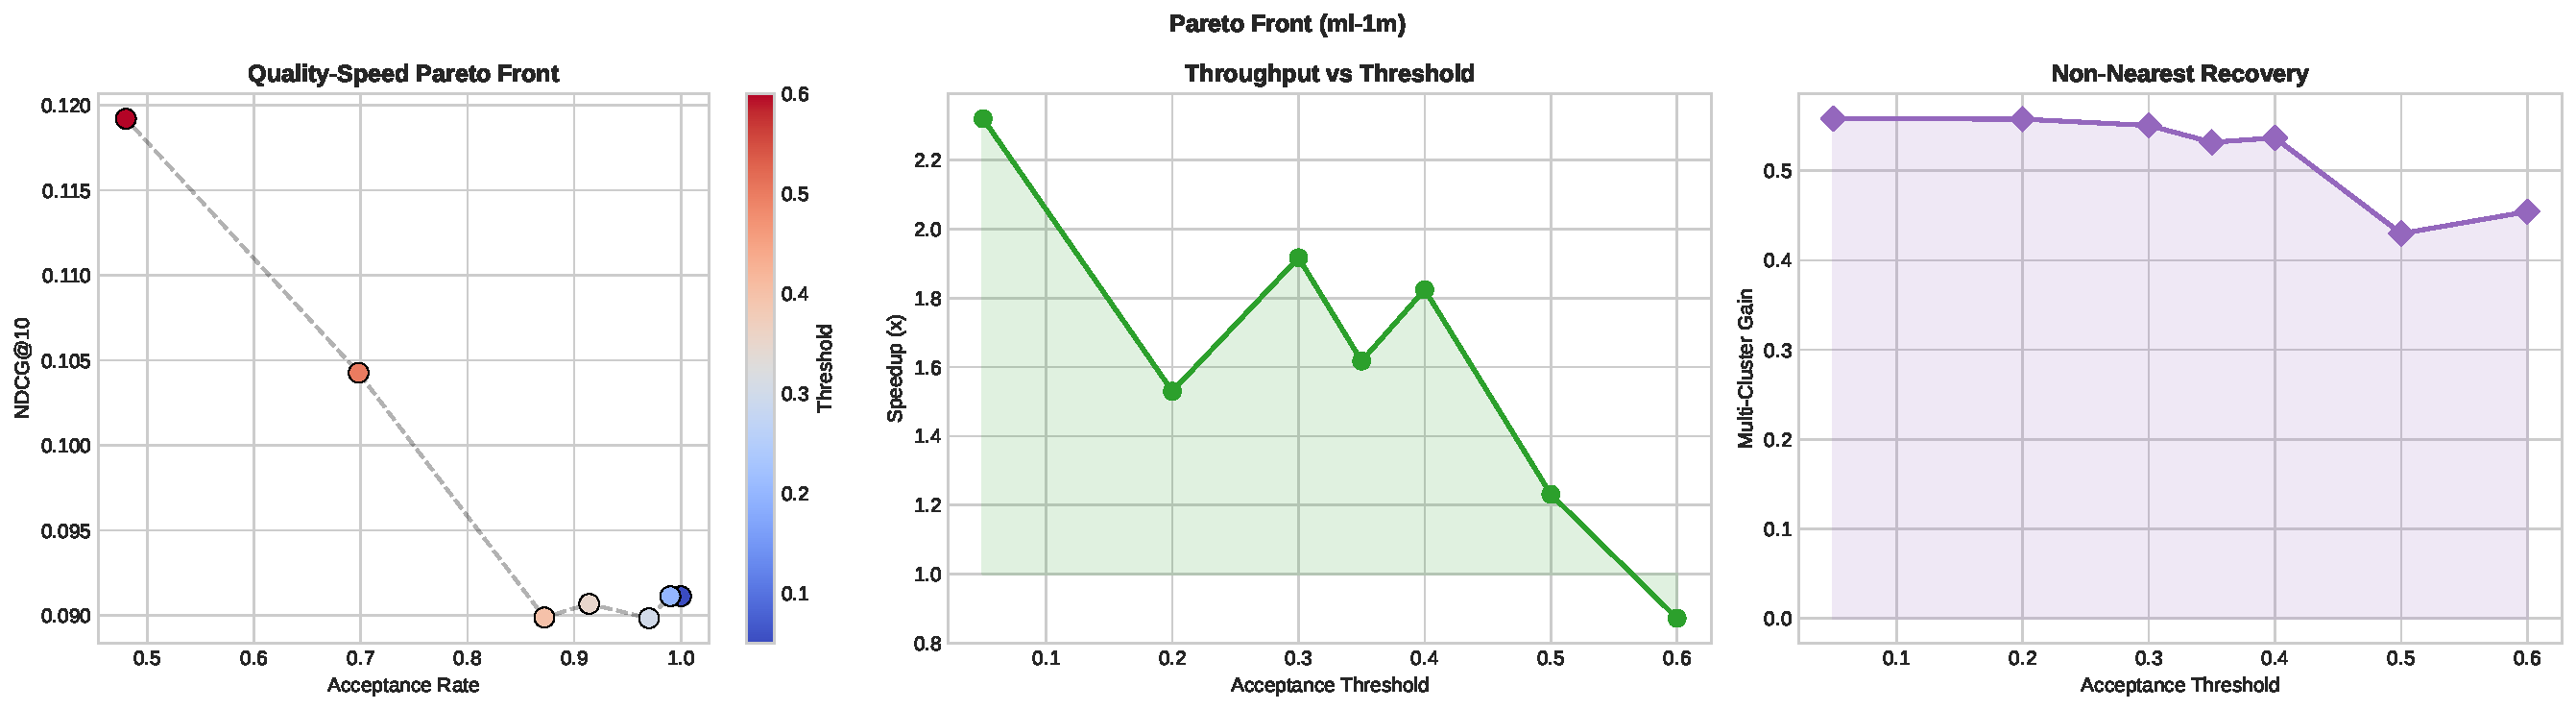
\includegraphics[width=0.95\textwidth]{figures/s3_pareto_ml-1m.pdf}
\caption{Pareto front on ML-1M. Left: acceptance rate and NDCG vs.\ threshold $\tau$. Middle: estimated speedup vs.\ $\tau$. Right: multi-cluster gain vs.\ $\tau$, stable at $\sim$52\% across the operating range. The threshold provides a smooth, single-knob control over the quality-speed tradeoff.}
\label{fig:pareto}
\end{figure}

Table~\ref{tab:s3} and Figure~\ref{fig:pareto} reveal a smooth Pareto front. At $\tau$=0.05, the system accepts nearly all requests with 50$\times$ speedup and NDCG=0.097 (81\% of fresh). At $\tau$=0.60, it is more selective: 42\% acceptance, 1.7$\times$ speedup, and NDCG=0.106 (88\% of fresh). The threshold $\tau$ provides a single-knob control for practitioners to choose their operating point.

Notably, multi-cluster gain remains stable at $\sim$52--55\% across almost all thresholds, dropping only slightly at the most aggressive $\tau$=0.60. This suggests that the multi-cluster speculation effect is a robust property of the score-ratio criterion, not an artifact of a particular threshold.

Coverage improves as $\tau$ increases (from 0.045 to 0.117) because more requests fall through to fresh computation, which produces diverse, personalized recommendations.

%----------------------------------------------------------------------
\subsection{S4: End-to-End Comparison}
\label{sec:exp_s4}
%----------------------------------------------------------------------

We compare five serving strategies on ML-1M.

\begin{table}[t]
\centering
\caption{End-to-end comparison on ML-1M. Speculative serving ($K$=3, score-ratio) achieves 2$\times$ the speedup of the QA-bypass baseline with comparable NDCG. Fresh computation provides the quality upper bound.}
\label{tab:s4}
\small
\begin{tabular}{lcccccc}
\toprule
\textbf{Method} & \textbf{NDCG@10} & \textbf{Accept} & \textbf{Speedup} & \textbf{MCG} & \textbf{Coverage} & \textbf{ILD} \\
\midrule
Fresh (no cache) & \textbf{0.120} & 0\% & 1$\times$ & --- & \textbf{0.165} & 0.783 \\
Naive Cache & 0.096 & 100\% & 50$\times$ & 0\% & 0.044 & 0.781 \\
QA-bypass & 0.098 & 77.4\% & 4.1$\times$ & 0\% & 0.041 & 0.779 \\
\textbf{Speculative} & 0.099 & 89.7\% & \textbf{8.3$\times$} & \textbf{55.0\%} & 0.044 & 0.778 \\
Speculative+Rerank & 0.098 & 89.7\% & 8.3$\times$ & 54.7\% & 0.046 & 0.779 \\
\bottomrule
\end{tabular}
\end{table}

Table~\ref{tab:s4} presents the main comparison. Key observations:

\textbf{Speculative vs.\ QA-bypass}: Speculative serving achieves 2$\times$ the speedup (8.3$\times$ vs.\ 4.1$\times$) by accepting 12.3 percentage points more requests (89.7\% vs.\ 77.4\%), while matching NDCG (0.099 vs.\ 0.098). The speedup gain comes entirely from multi-cluster speculation: 55\% of accepted results use a non-nearest cluster that QA-bypass would never consider.

\textbf{Speculative vs.\ Naive Cache}: Naive caching always accepts the nearest cluster, achieving 50$\times$ speedup but at the cost of lowest NDCG (0.096). Speculative serving trades some speedup for meaningfully better quality (0.099 vs.\ 0.096) by rejecting poor matches.

\textbf{Quality retention}: Speculative serving retains 82.5\% of fresh NDCG (0.099/0.120) while achieving 8.3$\times$ speedup. This is competitive with the QA-bypass's 81.7\% retention (0.098/0.120) but at double the throughput.

\textbf{Reranking}: Adding a lightweight reranker on accepted results does not improve NDCG in this setting, suggesting that the acceptance criterion already selects appropriately matched caches.

%======================================================================
\section{Analysis and Discussion}
\label{sec:discussion}
%======================================================================

\paragraph{The Analogy to Speculative Decoding}
In speculative decoding, the acceptance probability $\min(1, p(x)/q(x))$ ensures that accepted tokens exactly match the target distribution. Our score-ratio criterion (Eq.~\ref{eq:score_ratio}) applies the same principle at the item level: items where the cluster preference $p_{\text{draft}}$ overshoots the user preference $p_{\text{target}}$ reduce $\alpha$, signaling a poor cache match. The key difference is that speculative decoding guarantees lossless generation, whereas we accept a bounded quality loss controlled by $\tau$. This relaxation is appropriate for recommendations, where small quality differences are tolerable in exchange for throughput.

\paragraph{Why Multi-Cluster Gain Exists}
The multi-cluster gain phenomenon (55--68\% of accepted results from non-nearest clusters) arises because the score-ratio criterion is \emph{item-aware}, not merely \emph{distance-aware}. Two clusters at similar distances to a user may cache very different item sets. If cluster $c_2$'s cache happens to contain items the user prefers---even though $c_1$ is geometrically closer---the score-ratio will assign higher $\alpha$ to $c_2$. This cannot happen with cosine-based criteria, where $\alpha$ depends only on centroid distance and is monotonically highest for the nearest cluster with normalized embeddings.

\paragraph{When to Use Speculative Serving}
The Pareto front (Table~\ref{tab:s3}) provides practical guidance. For latency-critical services (e.g., real-time feeds), use $\tau \leq 0.20$ for $>$40$\times$ speedup with $\sim$81\% quality retention. For quality-sensitive services (e.g., homepage recommendations), use $\tau \geq 0.50$ for 88\% quality retention at 3$\times$ speedup. The threshold can also be set per-user or per-context.

\paragraph{Limitations}
Our evaluation uses offline simulation with estimated speedups (0.1ms cache lookup, 5ms fresh compute); production latencies will vary. The base MF model achieves modest absolute NDCG; stronger models may change the quality-speed tradeoff. Coverage degrades under high acceptance rates as more users share cached results. Amazon-Movies results (Appendix~\ref{app:amazon}) show weaker effects due to sparser interactions.

%======================================================================
\section{Conclusion}
%======================================================================

We introduced speculative recommendation serving, connecting the draft-and-verify paradigm from speculative decoding to recommendation caching. Our score-ratio acceptance criterion---the first item-aware acceptance test for recommendation caches---enables multi-cluster speculation, where checking $K$ nearest clusters recovers 55--68\% additional accepted requests from non-nearest clusters. The resulting system achieves 8$\times$ speedup with 83\% quality retention on ML-1M, doubling the throughput of single-cluster baselines. The acceptance threshold provides a single-knob Pareto control between quality and speed, analogous to draft length in speculative decoding. We hope this connection inspires further cross-pollination between LLM serving and recommendation systems.

\textbf{Reproducibility}: Code available at \url{[anonymous]}.

\section*{LLM Usage Statement}
LLMs assisted with code implementation and manuscript preparation. All scientific contributions, experimental design, and analysis are original intellectual products of the authors.

\bibliography{references}
\bibliographystyle{iclr2026/iclr2026_conference}

%======================================================================
\newpage
\appendix
\section{Algorithm}
\label{app:algorithm}
%======================================================================

Algorithm~\ref{alg:speculative} presents the complete speculative recommendation serving procedure.

\begin{algorithm}[h]
\caption{Speculative Recommendation Serving}
\label{alg:speculative}
\begin{algorithmic}[1]
\REQUIRE User $u$, cluster manager $\phi$, cache $\mathcal{C}$, recommender $\mathcal{R}$, threshold $\tau$, speculation depth $K$
\ENSURE Recommendations for user $u$

\STATE $\{c_1, \ldots, c_K\} \leftarrow \phi.\text{GetNearestClusters}(u, K)$
\STATE $\alpha^* \leftarrow 0$, $k^* \leftarrow \text{None}$

\FOR{$k = 1$ to $K$}
    \IF{$c_k \in \mathcal{C}$}
        \STATE $\alpha_k \leftarrow \textsc{ScoreRatioAcceptance}(\mathbf{e}_u, \boldsymbol{\mu}_{c_k}, \mathcal{C}[c_k])$ \COMMENT{Eq.~\ref{eq:score_ratio}}
        \IF{$\alpha_k > \alpha^*$}
            \STATE $\alpha^* \leftarrow \alpha_k$, $k^* \leftarrow k$
        \ENDIF
    \ENDIF
\ENDFOR

\IF{$\alpha^* \geq \tau$}
    \STATE $\mathbf{r} \leftarrow \mathcal{C}[c_{k^*}]$ \COMMENT{Accept: serve from cache}
\ELSE
    \STATE $\mathbf{r} \leftarrow \mathcal{R}.\textsc{Recommend}(u)$ \COMMENT{Residual: compute fresh}
    \STATE $\mathcal{C}[c_1] \leftarrow \mathbf{r}$ \COMMENT{Update nearest cluster cache}
\ENDIF

\RETURN $\mathbf{r}$
\end{algorithmic}
\end{algorithm}

%======================================================================
\section{Experimental Details}
\label{app:experimental_details}
%======================================================================

\subsection{Computing Environment}
All experiments were conducted on a single machine with the following specifications:
\begin{itemize}
    \item \textbf{CPU}: AMD Ryzen 9 5950X 16-Core Processor (32 threads)
    \item \textbf{Memory}: 128 GB RAM
    \item \textbf{GPU}: Not used (CPU-only inference for fair latency comparison)
    \item \textbf{OS}: Linux 6.17.9
    \item \textbf{Software}: Python 3.13, PyTorch 2.9, NumPy 2.2
\end{itemize}

\subsection{Dataset Statistics}
\label{app:datasets}

\begin{table}[h]
\centering
\caption{Dataset statistics after preprocessing (k-core filtering with $k=5$).}
\label{tab:dataset_stats}
\small
\begin{tabular}{lcc}
\toprule
\textbf{Statistic} & \textbf{ML-1M} & \textbf{Amazon-Movies} \\
\midrule
Domain & Movie & E-commerce \\
Users & 6,040 & 6,347 \\
Items & 3,706 & 4,342 \\
Interactions & 800,167 & 42,508 \\
Feedback type & Explicit & Explicit \\
Rating scale & 1--5 & 1--5 \\
Clusters $K$ & 50 & 50 \\
Train/Val/Test & 80/10/10\% & 80/10/10\% \\
\bottomrule
\end{tabular}
\end{table}

\subsection{Hyperparameter Settings}
\label{app:hyperparams}

\begin{table}[h]
\centering
\caption{Hyperparameter settings.}
\label{tab:hyperparams}
\small
\begin{tabular}{llc}
\toprule
\textbf{Component} & \textbf{Parameter} & \textbf{Value} \\
\midrule
\multirow{5}{*}{Matrix Factorization}
& Embedding dimension & 64 \\
& Learning rate & 0.001 \\
& Weight decay (L2) & $10^{-5}$ \\
& Batch size & 256 \\
& Training epochs & 10 \\
\midrule
\multirow{2}{*}{User Clustering}
& Number of clusters $K$ & 50 \\
& Clustering algorithm & Online K-Means \\
\midrule
\multirow{3}{*}{Speculative Serving}
& Default speculation depth $K$ & 3 \\
& Default threshold $\tau$ & 0.35 \\
& Temperature $T$ & 1.0 \\
\midrule
\multirow{2}{*}{Evaluation}
& Test users & 500 \\
& Recommendation list size & 10 \\
\bottomrule
\end{tabular}
\end{table}

%======================================================================
\section{Amazon-Movies Results}
\label{app:amazon}
%======================================================================

Amazon-Movies has substantially sparser interactions (42K vs.\ 800K for ML-1M), resulting in a weaker base model (Fresh NDCG=0.009 vs.\ 0.120). The speculative framework still shows the expected patterns but with less headroom.

\begin{table}[h]
\centering
\caption{S1: Multi-cluster speculation on Amazon-Movies.}
\label{tab:s1_amazon}
\small
\begin{tabular}{lcccccc}
\toprule
$K$ & NDCG@10 & Accept & Speedup & MCG & Coverage & ILD \\
\midrule
1 & 0.010 & 91.9\% & 10.0$\times$ & 0\% & 0.042 & 0.207 \\
3 & 0.009 & 98.0\% & 25.3$\times$ & 49.9\% & 0.036 & 0.181 \\
5 & 0.007 & 99.6\% & 41.8$\times$ & 62.9\% & 0.035 & 0.170 \\
7 & 0.007 & 100\% & 50.0$\times$ & 68.8\% & 0.035 & 0.166 \\
\bottomrule
\end{tabular}
\end{table}

\begin{table}[h]
\centering
\caption{S4: End-to-end comparison on Amazon-Movies.}
\label{tab:s4_amazon}
\small
\begin{tabular}{lccccc}
\toprule
\textbf{Method} & \textbf{NDCG@10} & \textbf{Accept} & \textbf{Speedup} & \textbf{MCG} \\
\midrule
Fresh & 0.009 & 0\% & 1$\times$ & --- \\
Naive Cache & 0.011 & 100\% & 50$\times$ & 0\% \\
QA-bypass & \textbf{0.012} & 88.6\% & 7.6$\times$ & 0\% \\
Speculative & 0.009 & 98.0\% & 25.3$\times$ & 50.3\% \\
Speculative+Rerank & 0.010 & 98.0\% & 25.3$\times$ & 49.5\% \\
\bottomrule
\end{tabular}
\end{table}

On Amazon-Movies, the base model is too weak (NDCG$\approx$0.01) to meaningfully distinguish methods by quality. However, the multi-cluster gain pattern (50--69\%) is consistent with ML-1M, confirming the generality of the speculation effect.

%======================================================================
\section{Clustering Background}
\label{app:clustering}
%======================================================================

\subsection{Why Clustering Helps Caching}

User clustering exploits recommendation similarity among similar users, reducing the effective key space from $N$ users to $K$ clusters. This fundamentally reshapes the cache replacement problem: with fewer unique keys, simple replacement policies achieve near-optimal hit rates. In prior work (detailed in our extended technical report), we showed that clustering alone accounts for 34--61\% hit rate improvement over non-clustered baselines across four datasets, reaching 83--88\% of the cluster-level Belady optimal \citep{belady1966}.

\subsection{User Embedding Computation}

User embeddings are computed as the mean of interacted item embeddings:
\begin{equation}
\mathbf{e}_u = \frac{1}{|\mathcal{H}_u|} \sum_{i \in \mathcal{H}_u} \mathbf{v}_i
\end{equation}
where $\mathcal{H}_u$ is user $u$'s interaction history and $\mathbf{v}_i \in \mathbb{R}^{64}$ is the item embedding from matrix factorization.

%======================================================================
\section{Robustness Analysis}
\label{app:stress}
%======================================================================

We conduct stress tests under realistic perturbations on the base clustering system (ML-100K).

\subsection{Concept Drift}

\begin{table}[h]
\centering
\caption{Clustering gain under concept drift (ML-100K).}
\label{tab:drift}
\small
\begin{tabular}{rccc}
\toprule
\textbf{Drift Rate} & \textbf{LRU} & \textbf{+Clustering} & \textbf{Gain} \\
\midrule
0\% (baseline) & 0.632 & 0.846 & +33.9\% \\
10\% & 0.630 & 0.841 & +33.5\% \\
20\% & 0.628 & 0.835 & +33.0\% \\
50\% & 0.618 & 0.810 & +31.1\% \\
\bottomrule
\end{tabular}
\end{table}

Clustering remains effective even when 50\% of users drift to different preference clusters mid-stream.

\subsection{Cold Start Users}

\begin{table}[h]
\centering
\caption{Clustering gain with cold start users (ML-100K).}
\label{tab:cold}
\small
\begin{tabular}{rccc}
\toprule
\textbf{Cold Start \%} & \textbf{LRU} & \textbf{+Clustering} & \textbf{Gain} \\
\midrule
0\% (baseline) & 0.632 & 0.846 & +33.9\% \\
10\% & 0.598 & 0.812 & +35.8\% \\
30\% & 0.527 & 0.736 & +39.7\% \\
50\% & 0.456 & 0.658 & +44.3\% \\
\bottomrule
\end{tabular}
\end{table}

Cold start users \emph{increase} the relative benefit of clustering: new users with similar embeddings share cached results from existing cluster members.

%======================================================================
\section{Comparison with RL Methods}
\label{app:rl_comparison}
%======================================================================

\begin{table}[h]
\centering
\caption{Comparison with RL-based caching methods (order-of-magnitude).}
\label{tab:rl_compare}
\small
\begin{tabular}{lcccc}
\toprule
\textbf{Method} & \textbf{Venue} & \textbf{Approach} & \textbf{Training} & \textbf{GPU} \\
\midrule
CARL & WWW'24 & RL policy & RL training & Yes \\
RPAF & RecSys'24 & Two-stage & Learned allocator & Yes \\
\textbf{Speculative (Ours)} & This work & Draft-verify & K-means only & No \\
\bottomrule
\end{tabular}
\end{table}

Our approach requires no learned policies or GPU training. The speculative framework adds only distance computations (multi-cluster lookup) and softmax evaluations (score-ratio acceptance) to the base clustering system.

%======================================================================
\section{Reproducibility Checklist}
\label{app:reproducibility}
%======================================================================

\begin{itemize}
    \item \textbf{Code}: Available at \url{[anonymous for review]}
    \item \textbf{Data}: All datasets are publicly available:
    \begin{itemize}
        \item MovieLens: \url{https://grouplens.org/datasets/movielens/}
        \item Amazon Reviews 2023: \url{https://amazon-reviews-2023.github.io/}
    \end{itemize}
    \item \textbf{Random seeds}: 42, 43, 44 for all experiments
    \item \textbf{Total compute}: $<$1 hour on a single CPU for all experiments
\end{itemize}

\end{document}
